% ---------------------------------------------------

\documentclass[11pt, journal]{IEEEtran}
\usepackage{hyperref}
\usepackage{color}
\usepackage[pdftex]{graphicx}
\usepackage{amsmath,amssymb,amsfonts,amsxtra}
\usepackage{booktabs}
\usepackage{longtable}
\usepackage{tabularx}


% ---------------------------------------------------

\begin{document}

    % ---------------------------------------------------

    \title{
        ALAN: Autonomous Long-Range Aquatic Navigation Vessel \\ 
        {\normalsize (The V is silent.)}
    }
    \author{
        Charbel Salloum, 
        Connor Stevens, 
        Corbin Barney, 
        Harrison LeTourneau, 
        Jared Pratt
    }

    \maketitle

    % ---------------------------------------------------

    \begin{abstract}
    This paper describes the design and implementation of ALAN (Autonomous Long-Range Aquatic Navigation), a semi-autonomous sailboat intended for long-duration operation in open water environments. The vessel navigates between user-defined waypoints using wind-powered propulsion, requiring no human intervention during transit. This work addresses the challenge of building a low-cost autonomous sailing platform suitable for environmental monitoring and oceanographic data collection, where conventional motorized vessels are limited by fuel capacity and operational cost. The mechanical, electrical, and software subsystems are presented, along with an analysis of associated risks and mitigation strategies.
    \end{abstract}

    % ---------------------------------------------------

    % ---------------------------------------------------

\section{Introduction}
\label{sec:introduction}

% Problem Statement
Autonomous marine vessels have the potential to revolutionize environmental monitoring, oceanographic data collection, and maritime logistics by eliminating the need for crewed expeditions. However, existing solutions are often prohibitively expensive, reliant on motor-driven propulsion with limited range, or lack the robustness required for extended blue water operation. A low-cost, sail-powered autonomous vessel would enable persistent ocean presence for data collection without the fuel constraints and maintenance overhead of motorized platforms.

% Solution Space
Several approaches to autonomous sailing have been explored in both academic and commercial domains. The SailBot competition community has produced numerous small-scale autonomous sailboats, typically using cloth sails with servo-actuated sheets. Commercial efforts such as Saildrone employ rigid wingsails on large platforms for ocean research. University projects have explored various hull configurations, sail types, and control algorithms ranging from simple reactive controllers to machine learning approaches.

% Related Work
Prior autonomous sailboat projects have demonstrated the viability of GPS waypoint navigation combined with wind-aware path planning. The self-trimming wingsail concept, where a tail vane provides passive torque to rotate the main sail element, has been shown to minimize power consumption compared to motor-actuated sail systems. Trimaran hull designs offer superior stability over monohulls, which is critical for sensor platforms that must remain upright in varying sea states.

% Solution / Contribution
ALAN (Autonomous Long-Range Aquatic Navigation) is a semi-autonomous trimaran sailboat that navigates between user-defined waypoints without human intervention. The vessel employs a self-trimming rigid wingsail for propulsion, minimizing power draw while maximizing aerodynamic efficiency. A dual-core STM32H755 microcontroller running FreeRTOS manages real-time sensor fusion (GPS, IMU, magnetometer, wind vane) and control loops for rudder actuation. Long-range communication is achieved via LoRa radio at 915~MHz, enabling telemetry uplink and route update downlink from a ground station.

% Proposed Work
The scope of this project includes:
\begin{itemize}
    \item Hull design and fabrication
    \item Keel and rudder construction
    \item Rigid wingsail with self-trimming mechanism
    \item Sensor integration for navigation and orientation
    \item Long-range wireless communication
    \item Embedded firmware for autonomous waypoint navigation
\end{itemize}
Excluded from scope are solar charging, full blue-water endurance testing, and machine-learning-based control. At Demo Day, the vessel will demonstrate autonomous navigation between a series of waypoints on open water (This will be done before hand and displayed using video).

% ---------------------------------------------------

    % ---------------------------------------------------

\section{Safety, Global, Societal, Ethical Considerations}
\label{sec:impact}

% Public Health, Safety and Welfare
The ALAN vessel operates autonomously on open water, presenting potential hazards to other watercraft, swimmers, and marine wildlife. To mitigate collision risk, the vessel will be limited to small, controlled bodies of water during testing and will transmit its GPS position continuously via LoRa for ground station monitoring. The vessel's low speed (sail-powered) and small size reduce the severity of any potential impact. Emergency recovery procedures allow the ground station operator to override autonomous control at any time.

% Environmental Factors
An autonomous sailboat is inherently environmentally friendly compared to motor-driven alternatives. Wind propulsion produces zero emissions and zero noise pollution underwater. The vessel uses a lithium-ion battery only for electronics, not propulsion, minimizing energy consumption. Materials selection (fiberglass, stainless steel, PLA) avoids toxic substances that could leach into water. 

% Global and Cultural Factors
Autonomous ocean monitoring platforms could democratize marine research by reducing the cost of data collection expeditions. Developing nations with extensive coastlines but limited research budgets could benefit significantly from low-cost autonomous sailing platforms. However, care must be taken to ensure that such technology is not misused for illicit activities (e.g., smuggling) or deployed in protected marine areas without proper authorization.

% Economic Factors
The project demonstrates that autonomous sailing vessels can be constructed at a fraction of the cost of commercial alternatives. Currently the only custom part is the hull and its associated components. By using off-the-shelf components (STM32 dev boards, commodity sensors, etc.), the total bill of materials remains accessible to other university teams and hobbyist developers.

% Professional Ethical Obligations
As engineers, the team has an obligation to ensure the vessel cannot cause harm to people or the environment. This includes implementing fail-safe behaviors (return-to-home on communication loss), clearly marking the vessel as unmanned, and operating only in permitted waterways. Data collected by onboard sensors will be handled responsibly, and the communication protocol will not interfere with other ISM band users beyond regulatory limits.

% ---------------------------------------------------

    \input{sections/tasks.tex}
    % ---------------------------------------------------

\section{Risks}
\label{sec:risks}

% ---------------------------------------------------

\subsection{Mechanical Risks}

\textcolor{riskgreen}{\textbf{Hull Integrity Failure:}} The fiberglass hull may develop cracks or delamination during operation, leading to water ingress and sinking. Mitigation: apply multiple layers of fiberglass (7 sheets, approximately 1~mm thickness) with additional reinforcement at stress points (keel mount, stern). Perform water submersion tests before open-water deployment.

\textcolor{riskgreen}{\textbf{Keel Detachment:}} The fin keel with steel-filled bulb experiences significant lateral forces during sailing. If the mounting bracket fails, the vessel loses stability and capsizes. Mitigation: use 304 stainless steel plate for mounting brackets with three 1/4-in bolts and lock nuts; reinforce the hull keel mount area with extra fiberglass layers and an embedded metal plate inside the boat.

\textcolor{riskgreen}{\textbf{Rudder Bearing Seizure:}} Salt water and debris may cause the rudder shaft bearings to seize, resulting in loss of steering. Mitigation: use ceramic ball bearings (R188) rated for marine environments; apply marine silicone grease; design for easy field replacement.

\textcolor{riskyellow}{\textbf{Mast/Sail Damage:}} High winds could overload the wingsail structure, snapping the mast or cracking the foam panels. Mitigation: design for expected wind conditions with safety margin; the self-trimming mechanism naturally feathers the sail in excessive wind.

% ---------------------------------------------------

\subsection{Electrical Risks}

\textcolor{riskgreen}{\textbf{Water Ingress to Electronics:}} Despite the sealed enclosure (Pelican M60), wave action or submersion during capsize could introduce water to the electronics bay. Mitigation: use IP-rated connectors for all cable pass-throughs; apply conformal coating to PCBs; include moisture-indicating desiccant packs. For any electronics that must be mounted externally (e.g., servos and antennas), use waterproof components and housings.

\textcolor{riskyellow}{\textbf{Battery Failure:}} The 3S LiPo battery (11.1~V nominal) poses fire and explosion risk if overcharged, over-discharged, or punctured. Mitigation: integrate a dedicated BMS (Battery Management System) that prevents overcharge and deep discharge; house battery in a fire-resistant compartment within the Pelican case.

\textcolor{riskyellow}{\textbf{LoRa Communication Loss:}} Environmental interference or antenna damage could sever the communication link. Mitigation: use high-gain 10~dBi antennas; implement autonomous return-to-home behavior on communication timeout; store mission parameters locally so the vessel can continue operation without uplink.

\textcolor{riskgreen}{\textbf{Servo Failure:}} The rudder or sail servo may burn out under sustained load. Mitigation: select waterproof, high-torque servos (20~kg-cm) rated for continuous duty; implement current monitoring to detect stall conditions.

% ---------------------------------------------------

\subsection{Software Risks}

\textcolor{riskgreen}{\textbf{Sensor Fusion Divergence:}} GPS, IMU, and magnetometer readings may conflict due to electromagnetic interference or sensor drift, causing incorrect heading calculations. Mitigation: implement complementary filtering; validate sensor readings against expected ranges; fall back to GPS-only navigation if IMU data is unreliable.

\textcolor{riskgreen}{\textbf{Real-Time Deadline Miss:}} FreeRTOS task scheduling may fail to meet control loop deadlines under heavy sensor polling load, causing unstable rudder behavior. Mitigation: assign appropriate task priorities; profile worst-case execution times; use the dual-core STM32H755 to distribute workload across CM7 (control) and CM4 (communication/telemetry) cores.

\textcolor{riskyellow}{\textbf{Path Planning Edge Cases:}} The navigation algorithm may fail to handle situations such as sailing directly into the no-sail zone ($\pm45^{\circ}$ into the wind), requiring tacking maneuvers that the path planner must handle correctly. Mitigation: implement a state machine with explicit tacking/jibing states; test extensively in simulation before on-water trials.

\textcolor{riskgreen}{\textbf{Path Planning Impossible:}} The path planner may fail to find a viable route to the waypoint due to obstacles or unfavorable wind conditions. Mitigation: implement a timeout for path planning; if no solution is found, switch to a safe loitering behavior until conditions improve, if conditions do not improve after a set length of time, return to home.

% ---------------------------------------------------

    % ---------------------------------------------------

\section{Schedule}
\label{sec:schedule}

% NOTE: No specific schedule with dates was found in the base documents.
% The following is a general milestone structure based on the task decomposition.
% Please update with actual dates and responsible parties.

\begin{table}[h]
\centering
\caption{Project Milestones}
\begin{tabular}{|p{0.35\linewidth}|p{0.25\linewidth}|p{0.3\linewidth}|}
\hline
\textbf{Milestone} & \textbf{Responsible} & \textbf{Deliverable} \\
\hline
Hull mold printed and surface-finished & Harrison LeTourneau & Smooth, release-coated female mold \\
\hline
Hull fiberglass layup complete & Harrison LeTourneau & Cured fiberglass hull shell \\
\hline
Keel and rudder fabricated & Team (Mechanical) & Assembled keel with bulb; rudder with shaft and bearings \\
\hline
Wingsail fabricated & Charbel Salloum, Connor Stevens & Foam-core fiberglass sail with tail mechanism \\
\hline
Electronics integration & Harrison LeTourneau, Jared Pratt & STM32H7 with all sensors and servos wired \\
\hline
LoRa communication verified & Harrison LeTourneau, Jared Pratt & Bidirectional link between vessel and ground station \\
\hline
Firmware: sensor polling and control loops & Corbin Barney & FreeRTOS tasks running on CM7 core \\
\hline
Firmware: navigation and path planning & Corbin Barney & Waypoint following with tacking logic \\
\hline
Full system integration & All & Complete vessel with all subsystems operational \\
\hline
On-water testing and Demo Day & All & Autonomous waypoint navigation demonstration \\
\hline
\end{tabular}
\end{table}

% ---------------------------------------------------

    % ---------------------------------------------------

\section{Conclusion}
\label{sec:conclusion}

The ALAN project demonstrates the feasibility of constructing a low-cost autonomous sailboat using accessible manufacturing techniques and off-the-shelf electronic components. By combining a trimaran hull design with a self-trimming rigid wingsail, the vessel achieves propulsion efficiency without the power consumption of motor-driven sail actuation. The use of a dual-core STM32H755 running FreeRTOS provides the real-time performance required for sensor fusion and control, while LoRa radio enables long-range communication suitable for open-water operation.

Key contributions of this project include: a fiberglass hull manufacturing process using 3D-printed molds accessible to university fabrication labs; a modular mechanical design allowing independent development and testing of keel, rudder, and sail subsystems; and an embedded software architecture distributing navigation and communication across dual processor cores.

Future work includes integration of solar charging for extended mission duration, implementation of machine-learning-based path planning for complex wind conditions, full blue-water endurance testing, and expansion of the sensor suite for environmental data collection applications. The modular design of ALAN facilitates iterative improvement across all subsystems.

% ---------------------------------------------------


    % ---------------------------------------------------

    \appendices
    % ---------------------------------------------------

\section{Sailboat Anatomy}
\label{app:sailboat_anatomy}

A sailboat consists of several key structural and functional components:

\begin{center}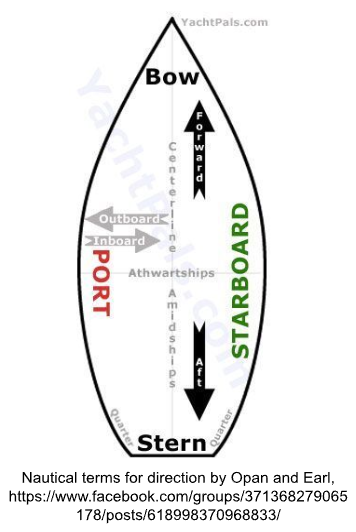
\includegraphics[width=0.6\columnwidth]{figures/images/boatAnatomy_directions.png}\end{center}

\textbf{Directions \& Regions:} Fore (forward) and aft (rearward) define movement along the longitudinal axis. Outboard (away from centerline) and inbaord (towards center line) refers to movement along the latitudinal axis. Bow is the front of the hull; stern is the rear. Starboard is the right side when facing forward; port is the left. 

\begin{center}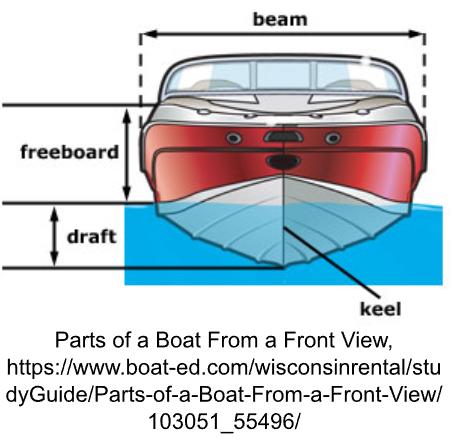
\includegraphics[width=0.6\columnwidth]{figures/images/boatAnatomy_waterLine.png}\end{center}

\textbf{Freeboard \& Draft:} Freeboard is the distance from the waterline to the deck. Draft is the distance from the waterline to the lowest point of the keel.

\begin{center}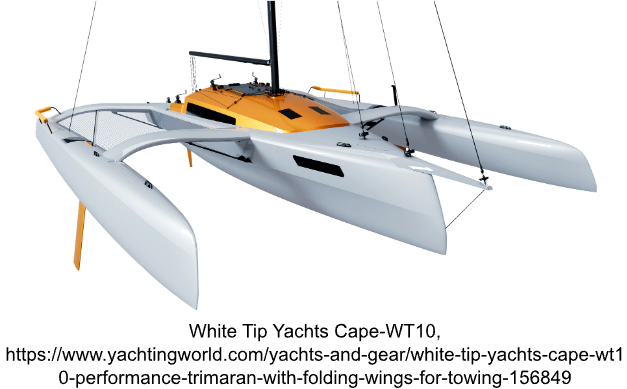
\includegraphics[width=0.6\columnwidth]{figures/images/Trimaran.png}\end{center}

\textbf{Hull:} The main body of the vessel providing buoyancy. Hull types include displacement hulls (slower, more stable) and planing hulls (faster, less stable). ALAN uses a trimaran configuration: a central vaka (main hull) with two amas (outriggers) connected by arms, providing exceptional stability.

\begin{center}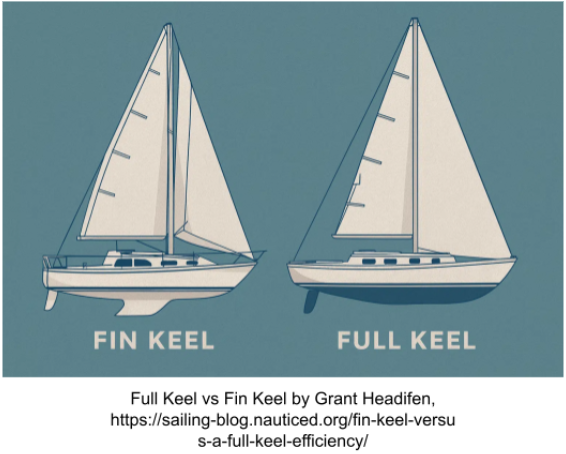
\includegraphics[width=0.6\columnwidth]{figures/images/boatAnatomy_keels.png}\end{center}

\textbf{Keel:} A fin extending below the hull that provides lateral resistance, preventing the boat from sliding sideways under sail force. Keel types include full keels (more stable, shallow draft, higher drag) and fin keels (more efficient, deeper draft). Sub-forms include squared, rounded, and bulb profiles. ALAN uses a fin keel with a bulb for stability and low center of mass.

\begin{center}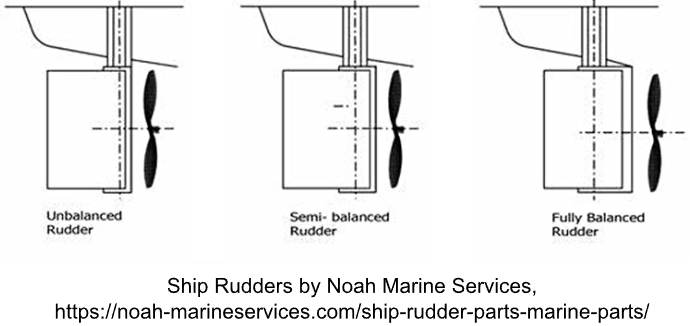
\includegraphics[width=0.6\columnwidth]{figures/images/boatAnatomy_rudders.png}\end{center}

\textbf{Rudder:} A movable fin at the stern used for steering. Balanced rudders are easy to turn but do not self-center; unbalanced rudders self-center but require more force. Styles include spade (free-floating, simple) and skeg-mounted (more protected, more stable). ALAN uses a spade rudder for simplicity.

\begin{center}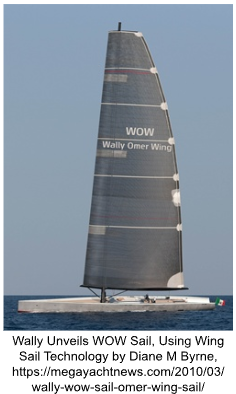
\includegraphics[width=0.6\columnwidth]{figures/images/boatAnatomy_wingSails.png}\end{center}

\textbf{Mast \& Sail:} The mast is a vertical bar supporting the sail. Sail materials include cloth (cheaper, traditional, more wear) and rigid (durable, more efficient lift). Autonomous boats favor rigid sails for durability.

\begin{center}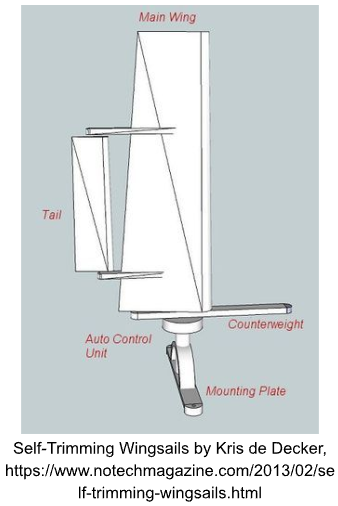
\includegraphics[width=0.6\columnwidth]{figures/images/selfTrimmingWingSail.png}\end{center}

\textbf{Self-Trimming Wingsail:} A rigid sail with a main element and a tail on a long rod aft of the pivot point. The tail provides passive aerodynamic torque to rotate the sail to the optimal angle. This design minimizes power consumption at the cost of higher mechanical complexity and wind-dependent response time.

% ---------------------------------------------------

    % ---------------------------------------------------

\section{Sailboat Physics}
\label{app:sailboat_physics}

\textbf{Lift Forces:} A sailboat is driven by two opposing lift forces. The sail generates lift from the wind, directed roughly perpendicular to the sail surface. The keel generates an opposing lateral lift force from the water. The net effect of these two forces propels the boat forward.

\textbf{Point of Sail:} The point of sail is the boat's angle relative to the wind direction. The angle of attack is the sail's angle relative to the apparent wind. The optimal angle of attack depends on the point of sail. The no-sail zone encompasses approximately $\pm45^{\circ}$ directly into the wind ($90^{\circ}$ total arc), where the sail cannot generate useful lift.

\textbf{Rudder Control:} The rudder modifies the interaction between sail and keel forces to change heading. Turning the rudder toward the wind decreases the effective keel force, causing the boat to turn away from the wind (bear away). Turning the rudder away from the wind increases the effective keel force, causing the boat to turn into the wind (head up).

\textbf{Center of Effort (COE) and Center of Lateral Resistance (CLR):} The COE is the point where the resultant sail lift force acts. The CLR is the point where the resultant keel/hull lateral resistance acts. When the COE is positioned slightly aft of the CLR, the boat exhibits weather helm---a natural tendency to turn into the wind. Weather helm is desirable because it provides inherent stability: if the helm is released, the boat rounds up into the wind and the sails luff, bringing the boat to a safe stop rather than accelerating uncontrolled.

% ---------------------------------------------------

    % ---------------------------------------------------

\section{Teams}
\label{app:teams}

We divided our group into several sub-teams in order to better divide work. In addition to this, we also contracted additional people for specific tasks.

% ---------------------------------------------------

\subsection{Additional Contributors}

Adam Welsh is a Computer Engineering student at the University of Utah that assisted the LoRa team in development.

Derek Tinoco is a Computer Scientist that assisted in the early sensor integration process.

Aliou Tippett is a student at the University of Utah that assisted the LoRa team in development.

% ---------------------------------------------------

\subsection{Sub-Teams}

LoRa Team: Harrison LeTourneau, Jared Pratt, Adam Welsh, Aliou Tippett. This team was responsible for the design, implementation, and testing of the LoRa communication system between the vessel and the ground station.

Sensor Team: Corbin Barney, Charbel Salloum, Connor Stevens, Derek Tinoco. This team was responsible for selecting, integrating, and testing the various sensors (GPS, IMU, wind vane) used for navigation and state awareness.

ALAN Team: Corbin Barney, Charbel Salloum, Connor Stevens, Harrison LeTourneau, Jared Pratt. This team was responsible for the overall integration of the vessel, including mechanical assembly, firmware development, and on-water testing.

Embedded Team: Corbin Barney, Charbel Salloum, Connor Stevens, Harrison LeTourneau, Jared Pratt, Derek Tinoco, Adam Welsh, Aliou Tippett. This team was responsible for the preliminary test benches used to test the various components of the vessel, including the LoRa communication system and the sensor suite.

% ---------------------------------------------------
    % ---------------------------------------------------

\section{Acknowledgements}
\label{app:acknowledgements}

This report was written with the assistance of AI tools (Claude Opus 4.6) for drafting, editing, and formatting. The authors provided the initial content and structure, and AI was used to refine language, ensure clarity, and maintain consistency. All technical content, design decisions, and project management were performed by the ALAN team members. The team is responsible for all final content and takes full ownership of the report. 

% ---------------------------------------------------

    % ---------------------------------------------------

    % Special figures
    % ---------------------------------------------------

\begin{table*}[htbp]
\label{tab:bom_rudder}
\centering
\caption{Bill of Materials -- Rudder}
\footnotesize
\begin{tabular}{|p{3.45cm}|p{5.5cm}|p{2.2cm}|p{4.75cm}|}
\hline
\textbf{Category} & \textbf{Item} & \textbf{Status} & \textbf{Notes} \\
\hline
Rudder - Shaft & Shaft Bearing & & R188 Ceramic 1/4 x 1/2 x 3/16 in. \\
\hline
Rudder - Shaft & Rudder Shaft & & SS 304 Round Bar (0.25 in. x 12 in.) \\
\hline
Rudder - Shaft & Rudder Plate & & 304 SS plate 0.25 in. \\
\hline
Rudder - Shaft & Rudder Cross Bolt, Barrel Nut & Delivered & 3/16 in. x 3/4 in. Aluminum Binding Post \\
\hline
Rudder - Mounting & Mounting Bolts & Delivered & 1/4-20 x 1-1/2 in. Zinc Plated Hex Bolt \\
\hline
Rudder - Mounting & Mounting Nuts & Delivered & 1/4-20 SS Nylon Insert Stop Nut \\
\hline
Rudder - Mounting & Mounting Washers & Delivered & 1/4 in. SS Flat Washer \\
\hline
Rudder - Mounting & Rear Mounting Plate & & 304 SS plate 0.25 in. \\
\hline
Rudder - Servo & Marine silicone grease (1 oz) & & \\
\hline
Rudder - Servo & Marine epoxy resin (small kit) & & \\
\hline
Rudder - Servo & Servo-Shaft Coupler & Ordered & 25 Tooth Spline to 1/4 in. Round Bore \\
\hline
Rudder - Servo & Rudder Servo & Delivered & DS3218 MG Digital Servo \\
\hline
Rudder - Servo & Servo Bolt & Delivered & M4-0.7x30mm Hex Bolt \\
\hline
Rudder - Servo & Servo Bolt Nut & & M4 SS Lock Nut \\
\hline
Rudder & PLA Filament & Lab Provided & \\
\hline
\end{tabular}
\end{table*}

\begin{table*}[htbp]
\label{tab:bom_keel}
\centering
\caption{Bill of Materials -- Keel}
\footnotesize
\begin{tabular}{|p{3.45cm}|p{5.5cm}|p{2.2cm}|p{4.75cm}|}
\hline
\textbf{Category} & \textbf{Item} & \textbf{Status} & \textbf{Notes} \\
\hline
Keel & Carbon fiber cloth & & Cover for completed assembly \\
\hline
Keel & Epoxy resin kit & & For composite layup \\
\hline
Keel - Structure & Keel Post & & SS 304 Square Bar (0.5 in. x 7 in.) \\
\hline
Keel - Structure & Keel Mounting Bracket & & 304 SS plate 0.25 in. \\
\hline
Keel - Structure & Mounting Bolts & Delivered & 1/4-20 x 1-1/2 in. Zinc Plated Hex Bolt \\
\hline
Keel - Structure & Mounting Nuts & Delivered & 1/4-20 SS Nylon Insert Stop Nut \\
\hline
Keel - Structure & Mounting Washers & Delivered & 1/4 in. SS Flat Washer \\
\hline
Keel - Structure & Keel Bulb & & SS 304 Round Tube (2 in. x 8.5 in.) \\
\hline
Keel - Structure & Steel Balls & Lab Provided & Ballast \\
\hline
Keel - Fin & Keel Cross Bolt, Barrel Nut & Delivered & 3/16 in. x 3/4 in. Aluminum Binding Post \\
\hline
Keel - Fin & PLA Filament & Lab Provided & \\
\hline
\end{tabular}
\end{table*}

\begin{table*}[htbp]
\label{tab:bom_hull}
\centering
\caption{Bill of Materials -- Hull}
\footnotesize
\begin{tabular}{|p{3.45cm}|p{5.5cm}|p{2.2cm}|p{4.75cm}|}
\hline
\textbf{Category} & \textbf{Item} & \textbf{Status} & \textbf{Notes} \\
\hline
Hull - Mold & Standard PLA Bambu filament & Lab Provided & \\
\hline
Hull - Mold & Rustoleum Filler/Sandable Primer & Purchased & \\
\hline
Hull - Mold & SprayMax 2K Topcoat High Gloss Black & ECE Request & \\
\hline
Hull - Mold & PARTALL Paste \#2 Wax & Delivered & \\
\hline
Hull - Mold & PARTALL Film \#10 PVA & ECE Request & \\
\hline
Hull - Glassing & Fiberglass Cloth Roll & ECE Request & 4 oz plain weave, 50 in. wide \\
\hline
Hull - Glassing & Econostitch Peel Ply & Delivered & \\
\hline
Hull - Glassing & TotalBoat 5:1 Marine Epoxy Kit & ECE Request & \\
\hline
Hull - Tools & Chip Paint Brushes (1 in., 24 pack) & Delivered & \\
\hline
Hull - Tools & Resin Epoxy Mixing Cups (50 pcs) & Delivered & \\
\hline
Hull - Tools & 3M Dynatron Spreaders (3 pack) & Delivered & \\
\hline
Hull - Tools & Wet/Dry Sandpaper Assortment & Purchased & \\
\hline
Hull - PPE & 3M Half Facepiece Respirator & Delivered & \\
\hline
Hull - PPE & 3M P100 Cartridge/Filter & Delivered & \\
\hline
Hull - PPE & Nitrile Exam Gloves & Delivered & \\
\hline
\end{tabular}
\end{table*}

\begin{table*}[htbp]
\label{tab:bom_sail}
\centering
\caption{Bill of Materials -- Rigid Sail}
\footnotesize
\begin{tabular}{|p{3.45cm}|p{5.5cm}|p{2.2cm}|p{4.75cm}|}
\hline
\textbf{Category} & \textbf{Item} & \textbf{Status} & \textbf{Notes} \\
\hline
Rigid Sail & 6061 Aluminum Mast (3 ft) & & \\
\hline
Rigid Sail & 6061 Aluminum Mast (alt. source) & & Metal Supermarket \\
\hline
Rigid Sail & Foam (XPS Rigid Board) & & \\
\hline
Rigid Sail & Cardboard & & \\
\hline
\end{tabular}
\end{table*}

\begin{table*}[htbp]
\label{tab:bom_electronics}
\centering
\caption{Bill of Materials -- Electronics}
\footnotesize
\begin{tabular}{|p{3.45cm}|p{5.5cm}|p{2.2cm}|p{4.75cm}|}
\hline
\textbf{Category} & \textbf{Item} & \textbf{Status} & \textbf{Notes} \\
\hline
Electronics & STM32H7 Dev Board & Delivered & \\
\hline
Electronics & RS485 to UART Adapter & & \\
\hline
Electronics - Sensors & Wind Vane Direction Sensor & Delivered & \\
\hline
Electronics - Sensors & 9-DoF IMU \& Magnetometer & Delivered & BNO055 \\
\hline
Electronics - Sensors & GPS Module & Delivered & NEO-6 \\
\hline
Electronics - Actuators & High-Torque Servo (20 kg-cm) & & Waterproof \\
\hline
Electronics - Power & Solar Panel (10 W, 12 V) & & \\
\hline
Electronics - Power & LiPo Battery (11.1 V, 3S) & & \\
\hline
Electronics - Power & Buck Converters (DC-DC) & & \\
\hline
Electronics - Power & 5 V and 12 V PDB & & \\
\hline
Electronics - Power & Battery BMS & & Overcharge/discharge protection \\
\hline
Electronics - Wireless & Adafruit RFM95W LoRa (915 MHz) & Delivered & \\
\hline
Electronics - Wireless & Adafruit Feather RP2040 w/ RFM95 & Lab Provided & \\
\hline
Electronics - Wireless & uFL SMT Antenna Connector & Delivered & \\
\hline
Electronics - Wireless & SMA to uFL Adapter Cable & & Comes with antennas \\
\hline
Electronics - Wireless & 10 dBi Whip Antenna w/ Adapters & Delivered & \\
\hline
Electronics - Wireless & SMA Male-Female Extension (5 ft) & Delivered & \\
\hline
\end{tabular}
\end{table*}

\begin{table*}[htbp]
\label{tab:bom_miscellaneous}
\centering
\caption{Bill of Materials -- Miscellaneous}
\footnotesize
\begin{tabular}{|p{3.45cm}|p{5.5cm}|p{2.2cm}|p{4.75cm}|}
\hline
\textbf{Category} & \textbf{Item} & \textbf{Status} & \textbf{Notes} \\
\hline
Misc & S6005-2RS Bearing & & 25 mm ID, deck mast partner \\
\hline
Misc & Pelican M60 & & \\
\hline
\end{tabular}
\end{table*}

% ---------------------------------------------------
    % ---------------------------------------------------

\begin{table*}[htbp]
\centering
\caption{Project Gantt Chart}
\label{tab:gantt}
\footnotesize
\setlength{\tabcolsep}{2pt}
\newcommand{\gb}{\rule{0.85cm}{5pt}}
\begin{tabular}{|p{3.5cm}|c|c|c|c|c|c|c|c|c|c|c|c|}
\hline
\textbf{Task} & \textbf{Jan} & \textbf{Feb} & \textbf{Mar} & \textbf{Apr} & \textbf{May} & \textbf{Jun} & \textbf{Jul} & \textbf{Aug} & \textbf{Sep} & \textbf{Oct} & \textbf{Nov} & \textbf{Dec} \\
\hline
Hull & \gb & \gb & \gb & \gb & \gb & \gb & & & & & & \\
\hline
Sail & & \gb & \gb & \gb & \gb & \gb & \gb & & & & & \\
\hline
Rudder & & \gb & \gb & \gb & \gb & \gb & & & & & & \\
\hline
Keel & & \gb & \gb & \gb & \gb & \gb & & & & & & \\
\hline
Complete Boat & \gb & \gb & \gb & \gb & \gb & \gb & \gb & & & & & \\
\hline
LoRa & & & \gb & \gb & \gb & \gb & \gb & \gb & \gb & & & \\
\hline
Servos & & \gb & \gb & \gb & \gb & \gb & \gb & \gb & & & & \\
\hline
Sensors & & & \gb & \gb & \gb & \gb & \gb & \gb & \gb & & & \\
\hline
MCU & & & \gb & \gb & \gb & \gb & \gb & \gb & \gb & \gb & & \\
\hline
RC Boat & & & & \gb & \gb & \gb & \gb & \gb & \gb & & & \\
\hline
Positioning & & & & & & & & \gb & \gb & \gb & & \\
\hline
Self Trimming Wingsail & & & & & & & & \gb & \gb & \gb & & \\
\hline
Path Planning & & & & & & & & & \gb & \gb & \gb & \\
\hline
Emergency Recovery & & & & & & & & & & \gb & \gb & \\
\hline
Ground Station Interface & & & & & & & & \gb & \gb & \gb & & \\
\hline
Autonomous Sailboat & & & & & & & & & & \gb & \gb & \gb \\
\hline
\end{tabular}
\end{table*}

% ---------------------------------------------------


    % ---------------------------------------------------

    \bibliographystyle{IEEEtran}
    \bibliography{bibtex/bib/IEEEexample, bibtex/bib/neal}
    \begin{thebibliography}{9}

\bibitem{stekzer2012}
R.~Stekzer, "Autonomous Sailboat Navigation," Ph.D. dissertation, Center for Computational Intelligence, De Montfort University, Leicester, 2012. [Online]. Available: \url{https://files01.core.ac.uk/download/pdf/228200594.pdf}

\bibitem{saildrone}
Saildrone. [Online]. Available: \url{https://www.saildrone.com/}

\bibitem{noahmarine}
"Ship Rudder," Noah Marine Services. [Online]. Available: \url{https://noah-marineservices.com/ship-rudder-parts-marine-parts/}

\bibitem{sailwings}
"Self Trimming Wingsail---the Pulley/Cord Control System," Sailwings.net, 2026. [Online]. Available: \url{https://www.sailwings.net/pulleycord.html}

\bibitem{sailingcatamarans}
"Keels or Daggerboards, the Pros and Cons," Sailingcatamarans.com. [Online]. Available: \url{https://www.sailingcatamarans.com/index.php/articles/12-to-be-published-mainly-technical/53-keels-or-daggerboards-the-pros-and-cons} (accessed Mar.~22, 2026).

\bibitem{skene2001}
N.~L.~Skene, \emph{Elements of Yacht Design}. Dobbs Ferry, NY: Sheridan House, 2001.

\bibitem{sun2024}
Z.~Sun, A.~Feng, J.~Yu, W.~Zhao, and Y.~Huang, "Development of autonomous sailboat sails and future perspectives: A review," \emph{Renewable and Sustainable Energy Reviews}, vol.~207, no.~114918, Sep.~2024, doi: \url{https://doi.org/10.1016/j.rser.2024.114918}.

\end{thebibliography}


\end{document}

% ---------------------------------------------------
